\documentclass[aspectratio=169,11pt]{beamer}
\usepackage[T1]{fontenc}
\usepackage[utf8]{inputenc}
\usepackage{lmodern,amsmath,amssymb,graphicx,tikz}
\usetikzlibrary{arrows.meta,calc}
\usetheme{default}
\usefonttheme{serif}
\setbeamercolor{normal text}{fg=black,bg=white}
\setbeamercolor{structure}{fg=black}
\setbeamercolor{frametitle}{fg=black}
\setbeamercolor{title}{fg=black}
\setbeamertemplate{navigation symbols}{}
\setbeamertemplate{footline}[frame number]
\setbeamertemplate{itemize items}[circle]
\setbeamersize{text margin left=8mm,text margin right=8mm}
\setlength{\parskip}{5pt}
\newcommand{\cO}{\mathcal O}
\newcommand{\cI}{\mathcal I}
\newcommand{\cA}{\mathcal A}
\newcommand{\db}{\bar\partial}
\newcommand{\C}{\mathbb C}
\newcommand{\Pj}{\mathbb P}
\newcommand{\norm}[1]{\lVert#1\rVert}
\newcommand{\src}[1]{\par\vfill{\scriptsize #1\par}}
\author{Daniel Gonz\'alez Casanova Azuela}

\title{How sections give an embedding}
\subtitle{The geometric idea behind Kodaira's theorem}
\date{5 November 2026}
\begin{document}
\begin{frame}\titlepage\end{frame}

\begin{frame}{Coordinates up to a common scale}
A point of complex projective space is a nonzero tuple, up to scaling:
\[
[z_0:\cdots:z_m]=[\lambda z_0:\cdots:\lambda z_m],\qquad \lambda\ne0.
\]
For example, \([1:2]=[2:4]\).
\par\bigskip
Where \(z_0\ne0\), we have ordinary coordinates
\[
\left(\frac{z_1}{z_0},\ldots,\frac{z_m}{z_0}\right).
\]
Our goal is to give a complex manifold \(X\) such coordinates globally.
\end{frame}

\begin{frame}{Sections supply the coordinates}
A \textbf{line bundle} \(A\to X\) attaches a complex line to each point.\\
A \textbf{section} \(s\) chooses a vector \(s(x)\in A|_x\), holomorphically.
\par\bigskip
Choose global sections \(s_0,\ldots,s_m\). In a local frame, write \(s_j=f_je\).
\[
\Phi(x)=[f_0(x):\cdots:f_m(x)].
\]
Changing the frame multiplies every coefficient by the same nonzero number.
The projective point stays the same.
\end{frame}

\begin{frame}{Kodaira embedding theorem}
Let \(X\) be a compact complex manifold with a positive holomorphic line bundle \(L\).
For sufficiently large \(N\), sections of \(L^{\otimes N}\) give an embedding
\[
\boxed{\Phi:X\hookrightarrow\Pj^m.}
\]
\par\bigskip
An embedding realizes \(X\) as a complex submanifold of projective space.
\par\medskip
Today: what must those sections do?
\src{Positive means that some smooth Hermitian metric has positive curvature form \(i\Theta_L\).}
\end{frame}

\begin{frame}{Kunihiko Kodaira}
\begin{columns}[c]
\column{.36\textwidth}
\centering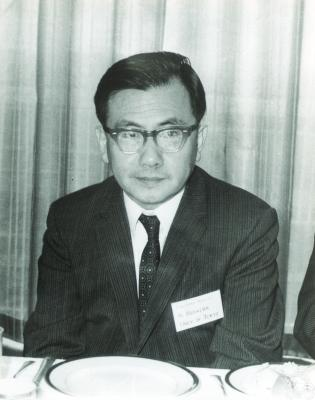
\includegraphics[height=4.8cm]{../assets/Kunihiko_Kodaira.png}
\column{.59\textwidth}
Kodaira received the Fields Medal in 1954.
\par\bigskip
His work connects complex geometry, analysis, and algebraic geometry.
\par\bigskip
Here, curvature provides the sections needed for an embedding.
\end{columns}
\src{Photo: Konrad Jacobs / MFO, Tokyo 1969, CC BY-SA 2.0 DE. Historical source: IAS scholar profile.}
\end{frame}

\begin{frame}{Three conditions on the sections}
\begin{center}
\renewcommand{\arraystretch}{1.9}
\begin{tabular}{ll}
Sections & Projective map\\\hline
No common zero (\textbf{base-point free}) & Defined everywhere\\
\textbf{Separate points} & Injective\\
\textbf{Separate tangent directions} & Immersion
\end{tabular}
\end{center}
\par\bigskip
For compact \(X\), an injective immersion is an embedding.
\end{frame}

\begin{frame}{Separating two points}
For distinct points \(x,y\), suppose we can choose sections \(s,t\) with
\[
\begin{array}{c|cc}
 & x & y\\\hline
s & 1 & 0\\
t & 0 & 1
\end{array}
\]
These values use chosen coordinates in the two fibres.
\par\bigskip
The tuples of section values at \(x\) and \(y\) cannot be proportional.
Therefore \(\Phi(x)\ne\Phi(y)\).
\end{frame}

\begin{frame}{Tangent directions must survive too}
\begin{columns}[c]
\column{.44\textwidth}
\centering
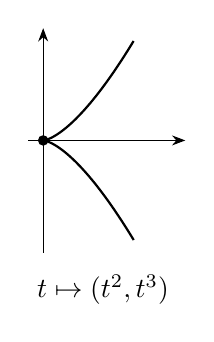
\begin{tikzpicture}[scale=.95,>=Stealth]
\draw[->] (-.2,0)--(1.9,0);
\draw[->] (0,-1.5)--(0,1.5);
\draw[thick,domain=-1.1:1.1,samples=70,variable=\t] plot ({\t*\t},{\t*\t*\t});
\fill (0,0) circle (2pt);
\node at (.8,-2) {\(t\mapsto(t^2,t^3)\)};
\end{tikzpicture}
\column{.53\textwidth}
This map is injective, but its derivative at zero vanishes.
\par\bigskip
We also need \(d\Phi_x(v)\ne0\) whenever \(v\ne0\).
\par\bigskip
Locally, this means that the ratios \(s_j/s_0\) detect every tangent direction.
\end{columns}
\src{The picture shows the real slice of the complex cusp.}
\end{frame}

\begin{frame}{Where vanishing enters}
We need global sections with prescribed values and first derivatives.
\par\bigskip
An exact sequence gives
\[
\underbrace{H^0(X,A)}_{\text{global sections}}
\longrightarrow
\underbrace{\text{prescribed data}}_{\text{values or first derivatives}}
\longrightarrow
\underbrace{H^1(X,A\otimes I)}_{\text{obstruction group}}.
\]
Here \(I\) records which local data we want to prescribe.
\[
\boxed{H^1(X,A\otimes I)=0\quad\Longrightarrow\quad
\text{every choice of data lifts}.}
\]
The analytic part of the proof establishes the required vanishing for large \(N\).
\end{frame}

\begin{frame}{The geometric mechanism}
\begin{enumerate}
\setlength{\itemsep}{14pt}
\item Vanishing lets us prescribe values and first derivatives.
\item These sections define an injective immersion.
\item Compactness gives an embedding into projective space.
\end{enumerate}
\par\bigskip
\centering\large Enough sections become global coordinates.
\end{frame}
\end{document}
